\documentclass{beamer}
\usepackage{amsfonts,amsmath,oldgerm}
\usepackage{ragged2e}

\usetheme{sintef}

\newcommand{\testcolor}[1]{\colorbox{#1}{\textcolor{#1}{test}}~\texttt{#1}}

\usefonttheme[onlymath]{serif}

\titlebackground*{assets/background}

\newcommand{\hrefcol}[2]{\textcolor{cyan}{\href{#1}{#2}}}

\title{Aula 01 - Software as a Service}
\subtitle{2023.1 - PDWA5 - Programação Dinâmica para Web}
\course{Tecnologia em Análise e Desenvolvimento de Sistemas}
\author{\href{mailto:luiz.quirino@ifsp.edu.br}{Luiz \textbf{Quirino}}}
\IDnumber{luiz.quirino@ifsp.edu.br}



\begin{document}
\maketitle

%\begin{frame}
%
%      Este material é produzido utilizando \LaTeX\, baseado na SINTEF Presentation, disponibilizado sob licenciamento \hrefcol{https://creativecommons.org/licenses/by-nc/4.0/legalcode}{Creative Commons CC BY 4.0}
%
%\vspace{\baselineskip}

%In the following you find a brief introduction on how to use \LaTeX\ and the beamer package to prepare slides, based on the one written by \hrefcol{mailto:federico.zenith@sintef.no}{Federico Zenith} for \hrefcol{https://www.overleaf.com/latex/templates/sintef-presentation/jhbhdffczpnx}{SINTEF Presentation}

% This template is released under \hrefcol{https://creativecommons.org/licenses/by-nc/4.0/legalcode}{Creative Commons CC BY 4.0} license
%\end{frame}
\footlinecolor{sintefdarkgreen}
\section{Introdução}
\begin{frame}
	\frametitle{SaaS - Software as a Service}

	\textbf{Definição:} Software as a Service (SaaS) é um modelo de entrega de software em que o software é acessado pela internet e normalmente licenciado por assinatura.




\end{frame}
\begin{frame}
	\frametitle{SaaS - Software as a Service}

	\textbf{Características do SaaS:}
	\begin{itemize}
		\item Acesso via internet: As aplicações SaaS são executadas diretamente no navegador web.
		\item Licenciado por assinatura: Os usuários pagam uma taxa periódica (mensal ou anual) pelo uso do serviço.
		\item Nenhuma instalação local necessária: Não é necessário instalar ou manter qualquer software no dispositivo do usuário.
		\item Manutenção centralizada: As atualizações e manutenções são realizadas pelo provedor do serviço na nuvem.
	\end{itemize}


\end{frame}

\begin{frame}
	\frametitle{SaaS no Modelo de Cloud Computing}

	SaaS é uma das três principais categorias do cloud computing, juntamente com Infrastructure as a Service (IaaS) e Platform as a Service (PaaS).



\end{frame}
\begin{frame}
	\frametitle{SaaS no Modelo de Cloud Computing}

	\textbf{Características do Modelo SaaS:}
	\begin{itemize}
		\item Gerenciamento simplificado: Os usuários não precisam gerenciar, instalar ou fazer upgrade de software; tudo é tratado pelo provedor do serviço.
		\item Acesso via internet: As aplicações SaaS são executadas diretamente no navegador web.
		\item Licenciado por assinatura: Os usuários pagam uma taxa periódica (mensal ou anual) pelo uso do serviço.
		\item Manutenção centralizada: As atualizações e manutenções são realizadas pelo provedor do serviço na nuvem.
	\end{itemize}


\end{frame}

\begin{frame}
	\frametitle{Benefícios do SaaS}

	Os benefícios do SaaS incluem:
	\linebreak
	\linebreak
	\textbf{Escalabilidade:} SaaS permite que as empresas escalem facilmente o uso de software de acordo com as necessidades do negócio.
	\linebreak
	\linebreak
	\textbf{Acessibilidade:} Como o SaaS é baseado na nuvem, ele pode ser acessado de qualquer lugar com uma conexão à internet.


\end{frame}

\begin{frame}
	\frametitle{Benefícios do SaaS}

	Os benefícios do SaaS incluem:
	\linebreak
	\linebreak
	\textbf{Escalabilidade:} SaaS permite que as empresas escalem facilmente o uso de software de acordo com as necessidades do negócio.
	\linebreak
	\linebreak
	\textbf{Acessibilidade:} Como o SaaS é baseado na nuvem, ele pode ser acessado de qualquer lugar com uma conexão à internet.

\end{frame}


\begin{frame}
	\frametitle{Modelo de Negócio SaaS}

	No modelo de negócio SaaS, os usuários pagam uma taxa recorrente, geralmente mensal ou anual, para acessar o software.

	\textbf{Vantagens do modelo de negócio SaaS:}

	\begin{itemize}
		\item Fluxo de receita previsível: A receita é gerada de forma constante, tornando o planejamento financeiro mais estável para o fornecedor.
		\item Acesso contínuo ao software: Os usuários podem continuar utilizando o software enquanto mantiverem a assinatura ativa.
	\end{itemize}
\end{frame}
\begin{frame}
	\frametitle{Modelo de Negócio SaaS}

	\textbf{Vantagens do modelo de negócio SaaS:}

	\begin{itemize}
		\item Atualizações e suporte inclusos: O fornecedor é responsável por manter o software atualizado e oferecer suporte técnico.
		\item Menor custo inicial: Os usuários não precisam fazer um grande investimento inicial para adquirir licenças de software.
	\end{itemize}


\end{frame}




\begin{frame}
	\frametitle{O Papel da Tecnologia da Informação em SaaS}

	A Tecnologia da Informação (TI) desempenha um papel crucial no modelo de negócio SaaS, assumindo diversas responsabilidades fundamentais:

	\begin{itemize}
		\item \textbf{Segurança:} Garantir a proteção dos dados dos usuários e a integridade do sistema contra ameaças cibernéticas.
		\item \textbf{Integração:} Realizar a integração do SaaS com outras soluções e sistemas utilizados pela empresa, permitindo a troca de dados e informações.
	\end{itemize}


\end{frame}
\begin{frame}
	\frametitle{O Papel da Tecnologia da Informação em SaaS}

	\begin{itemize}
		\item \textbf{Suporte ao Usuário:} Fornecer suporte técnico e resolver questões dos usuários relacionadas ao SaaS.
		\item \textbf{Disponibilidade e Desempenho:} Assegurar que o serviço SaaS esteja sempre disponível e funcione sem problemas, mantendo altos níveis de desempenho.
		\item \textbf{Implementação de APIs:} Desenvolver e implementar APIs que possibilitem a integração do SaaS com outros sistemas e aplicações.
	\end{itemize}


\end{frame}

\section{APIs e SaaS}

\begin{frame}
	\frametitle{O que são APIs}

	As APIs (Application Programming Interfaces) são interfaces de programação de aplicações que atuam como intermediárias entre diferentes softwares, permitindo a comunicação e a troca de dados de forma padronizada.


\end{frame}
\begin{frame}
	\frametitle{O que são APIs}


	\begin{itemize}
		\item As APIs permitem que aplicações se comuniquem e interajam entre si, mesmo que sejam desenvolvidas por diferentes empresas ou equipes.
		\item Elas fornecem um conjunto de regras e protocolos que definem como os programas podem se conectar e compartilhar informações.
		\item Com o uso de APIs, desenvolvedores podem acessar funcionalidades específicas de um software ou serviço sem precisar conhecer todos os detalhes internos do mesmo.
		\item As APIs são amplamente utilizadas para integrar diferentes sistemas e serviços, possibilitando a criação de aplicativos complexos e completos.
	\end{itemize}

\end{frame}


\begin{frame}
	\frametitle{APIs no contexto do SaaS}

	As APIs desempenham um papel fundamental no contexto do SaaS, permitindo a integração dos aplicativos SaaS com outros sistemas e aplicativos. Isso é essencial para a funcionalidade e a utilidade de muitos SaaS, pois permite que eles trabalhem em conjunto com outros softwares que uma empresa já esteja usando.


\end{frame}

\begin{frame}
	\frametitle{APIs no contexto do SaaS}

	\begin{itemize}
		\item As APIs possibilitam que os aplicativos SaaS acessem dados e funcionalidades de outros sistemas, permitindo a troca de informações e a sincronização de dados.
		\item Através das APIs, os aplicativos SaaS podem se integrar a sistemas internos da empresa, como sistemas de gerenciamento de vendas, finanças ou recursos humanos.
		\item Além disso, as APIs permitem que os desenvolvedores externos criem funcionalidades personalizadas para o SaaS, estendendo suas capacidades e adaptando-o às necessidades específicas dos usuários.
	\end{itemize}


\end{frame}

\begin{frame}
	\frametitle{Benefícios do uso de APIs em SaaS}

	O uso de APIs em SaaS oferece diversos benefícios que contribuem para a eficiência e produtividade das operações das empresas.

	\begin{itemize}
		\item \textbf{Interoperabilidade:} As APIs possibilitam a integração e comunicação entre diferentes softwares, permitindo que sistemas diversos trabalhem em conjunto. Isso torna os processos de negócios mais eficientes e facilita o compartilhamento de informações entre diferentes plataformas.
		\item \textbf{Automação:} Ao utilizar APIs, as empresas podem automatizar tarefas repetitivas, reduzindo a necessidade de intervenção manual. Isso leva a um aumento na produtividade, pois processos que anteriormente demandavam tempo e esforço manual agora podem ser executados automaticamente.
	\end{itemize}

\end{frame}

\begin{frame}
	\frametitle{Princípios Básicos de APIs em SaaS}

	Ao desenvolver APIs para SaaS, é fundamental considerar alguns princípios básicos que garantem a eficácia e a qualidade das interações entre os sistemas.
	\begin{itemize}
		\item \textbf{Desempenho:} As APIs devem ser otimizadas para fornecer respostas rápidas e eficientes. A minimização do tempo de resposta é essencial para proporcionar uma experiência de uso satisfatória.
		\item \textbf{Facilidade de Uso:} Uma API bem projetada deve ser fácil de usar e entender. Documentação clara e exemplos de código ajudam os desenvolvedores a implementarem a API de forma rápida e eficiente.
	\end{itemize}



\end{frame}

\begin{frame}
	\frametitle{Princípios Básicos de APIs em SaaS}

	\begin{itemize}
		\item \textbf{Desempenho:} As APIs devem ser otimizadas para fornecer respostas rápidas e eficientes. A minimização do tempo de resposta é essencial para proporcionar uma experiência de uso satisfatória.
		\item \textbf{Facilidade de Uso:} Uma API bem projetada deve ser fácil de usar e entender. Documentação clara e exemplos de código ajudam os desenvolvedores a implementarem a API de forma rápida e eficiente.
	\end{itemize}


\end{frame}

\begin{frame}
	\frametitle{APIs REST e SOAP: Uma Visão Geral}

	As APIs REST (Representational State Transfer) e SOAP (Simple Object Access Protocol) são duas abordagens comuns para a construção de APIs que facilitam a comunicação entre diferentes sistemas.

	\textbf{REST:}
	\begin{itemize}
		\item É um estilo arquitetônico que utiliza os métodos HTTP (GET, POST, PUT, DELETE) para realizar operações em recursos.
		\item É leve e utiliza uma estrutura simples para transferência de dados, geralmente no formato JSON ou XML.
		\item É amplamente utilizado em aplicações web e é conhecido por sua facilidade de uso e simplicidade.
	\end{itemize}
\end{frame}

\begin{frame}
	\frametitle{APIs REST e SOAP: Uma Visão Geral}
	\textbf{SOAP:}
	\begin{itemize}
		\item É um protocolo baseado em XML para a troca de mensagens entre sistemas.
		\item Utiliza especificações formais de mensagens e é mais complexo em comparação com REST.
		\item É comumente usado em sistemas corporativos e integrações entre diferentes plataformas.
	\end{itemize}

\end{frame}

\begin{frame}
	\frametitle{Arquitetura Cliente-Servidor em APIs}

	A arquitetura cliente-servidor é o modelo mais comum usado para conectar dispositivos via rede. No contexto de APIs, esse modelo é amplamente empregado para a troca de informações entre sistemas.

	\textbf{Funcionamento:}
	\begin{itemize}
		\item O \textbf{cliente} é o dispositivo ou aplicativo que envia solicitações para a API, buscando informações ou serviços específicos.
		\item O \textbf{servidor} é o componente que hospeda a API e responde às solicitações do cliente, fornecendo as informações solicitadas.
		\item A comunicação entre cliente e servidor ocorre através do protocolo HTTP, onde o cliente envia requisições (por exemplo, uma solicitação GET) e o servidor responde com os dados solicitados.
	\end{itemize}


\end{frame}

\begin{frame}
	\frametitle{Tokens de Acesso em APIs SaaS }

	Os tokens de acesso desempenham um papel importante na autenticação e autorização de solicitações de API em ambientes SaaS. Eles são utilizados para comprovar a identidade do usuário e garantir que apenas usuários autorizados tenham acesso aos recursos protegidos pela API.

	\textbf{Funcionamento:}
	\begin{itemize}
		\item Os tokens de acesso são emitidos após o usuário se autenticar com sucesso no sistema.
		\item Esses tokens são então passados junto com cada solicitação de API feita pelo usuário, geralmente como um cabeçalho HTTP ou parâmetro de consulta.
		\item Ao receber uma solicitação, a API verifica o token de acesso para garantir que ele seja válido e corresponda a um usuário autenticado e autorizado.
	\end{itemize}

\end{frame}

\begin{frame}
	\frametitle{Tokens de Acesso em APIs SaaS}

	\textbf{Funcionamento:}
	\begin{itemize}
		\item Os tokens de acesso também podem incluir informações sobre as permissões do usuário, permitindo que a API determine quais ações o usuário está autorizado a realizar.
	\end{itemize}

	\textbf{Exemplo prático:} Um exemplo popular de uso de tokens de acesso é o protocolo OAuth 2.0. Depois que um usuário se autentica com sucesso em um serviço, ele recebe um token de acesso. Esse token é incluído em todas as solicitações subsequentes feitas pelo aplicativo ou serviço em nome do usuário, garantindo que ele tenha acesso seguro aos recursos protegidos pela API.

\end{frame}

\begin{frame}
	\frametitle{Segurança em APIs para SaaS}

	A segurança é uma preocupação fundamental na criação e uso de APIs em ambientes SaaS. Para garantir a proteção dos dados e recursos sensíveis, é necessário implementar diversas medidas de segurança.

	\textbf{Considerações de segurança incluem:}
	\begin{itemize}
		\item \textbf{Autenticação:} Garantir que os usuários sejam corretamente autenticados antes de acessarem os recursos da API.
		\item \textbf{Autorização:} Controlar quais recursos e operações cada usuário pode acessar e executar.
		\item \textbf{Criptografia de dados:} Proteger a confidencialidade dos dados transmitidos através da API usando criptografia.
	\end{itemize}

\end{frame}
\begin{frame}
	\frametitle{Segurança em APIs para SaaS}

	\textbf{Considerações de segurança incluem:}
	\begin{itemize}
		\item \textbf{Limitação de taxa:} Implementar mecanismos de limitação de taxa para evitar ataques de negação de serviço (DDoS) ao restringir o número de solicitações que um cliente pode fazer em um determinado período.
		\item \textbf{Manuseio seguro de erros:} Garantir que mensagens de erro não revelem informações sensíveis e que não dêem pistas para potenciais atacantes.
	\end{itemize}

	É importante manter as APIs atualizadas e monitoradas para detectar qualquer atividade suspeita. A segurança em APIs é um aspecto crucial para proteger os dados e garantir a confiança dos usuários.

\end{frame}


\begin{frame}
	\frametitle{Planejamento de uma API para SaaS}

	\begin{itemize}
		\item Definição de dados e funcionalidades:
		      \begin{itemize}
			      \item Identificar requisitos e necessidades dos usuários.
			      \item Decidir quais dados e funcionalidades serão expostos pela API.
		      \end{itemize}

		\item Estruturação da API:
		      \begin{itemize}
			      \item Definir a organização dos endpoints e recursos.
			      \item Especificar os métodos HTTP suportados (GET, POST, PUT, DELETE).
		      \end{itemize}

		\item Protocolos e padrões:
		      \begin{itemize}
			      \item Escolher entre REST, SOAP ou outros protocolos para a API.
			      \item Implementar autenticação, como OAuth, para garantir segurança.
		      \end{itemize}
	\end{itemize}

\end{frame}
\begin{frame}
	\frametitle{Planejamento de uma API para SaaS (cont.)}

	\begin{itemize}
		\item Experiência do desenvolvedor:
		      \begin{itemize}
			      \item Criar documentação clara e completa da API.
			      \item Oferecer suporte para os desenvolvedores que utilizarem a API.
			      \item Facilitar o uso da API, tornando-a intuitiva e bem documentada.
		      \end{itemize}
	\end{itemize}

	Exemplo prático: Ao planejar a API do Twitter, a empresa decidiu expor dados e funcionalidades que permitiriam aos desenvolvedores criar uma variedade de aplicações diferentes, desde rastreamento de tópicos populares até análise de sentimentos.

\end{frame}

\begin{frame}{Documentação de API para SaaS}

	A documentação da API é crucial para os desenvolvedores que irão usar a API. Ela deve incluir informações sobre:

	\begin{itemize}
		\item Autenticação: Como autenticar as solicitações à API para garantir a segurança.
		\item Endpoints: O que cada endpoint faz e quais recursos estão disponíveis.
		\item Parâmetros: Quais parâmetros cada endpoint aceita e como utilizá-los corretamente.
		\item Respostas: Que tipo de resposta esperar da API e como interpretá-las.
		\item Exemplos de uso: Demonstração de casos de uso e exemplos de código para facilitar a implementação.
	\end{itemize}

	Uma boa documentação de API pode ser um fator decisivo para os desenvolvedores ao escolher entre diferentes APIs.

\end{frame}

\begin{frame}{Testando APIs para SaaS}

	Testar APIs envolve:

	\begin{itemize}
		\item Enviar diferentes tipos de solicitações à API.
		\item Verificar se as respostas estão de acordo com o esperado.
	\end{itemize}

	Tipos de testes incluem:

	\begin{itemize}
		\item Testes de Unidade: Testar a funcionalidade individual de cada endpoint.
		\item Testes de Integração: Testar como diferentes partes da API funcionam juntas.
		\item Testes de Carga: Testar como a API se comporta sob carga pesada de solicitações.
	\end{itemize}

\end{frame}

\begin{frame}{Exemplo Prático}

	Ferramentas como Postman ou Insomnia são frequentemente usadas para testar APIs. Elas permitem que os desenvolvedores enviem solicitações e vejam as respostas em tempo real, facilitando o processo de testes.

\end{frame}


\begin{frame}{Manutenção e Evolução de APIs para SaaS}

	\textbf{Manutenção da API}

	\begin{itemize}
		\item Monitorar a API para detectar problemas e bugs.
		\item Garantir que a API esteja sempre disponível e funcionando corretamente.
	\end{itemize}

	\textbf{Evolução da API}

	\begin{itemize}
		\item Adicionar novos recursos e funcionalidades.
		\item Melhorar a funcionalidade existente.
		\item Eventualmente, depreciação de partes da API.
	\end{itemize}

\end{frame}







\begin{frame}[fragile]{Imagem do dia}

	\begin{figure}[H]
		\centerline{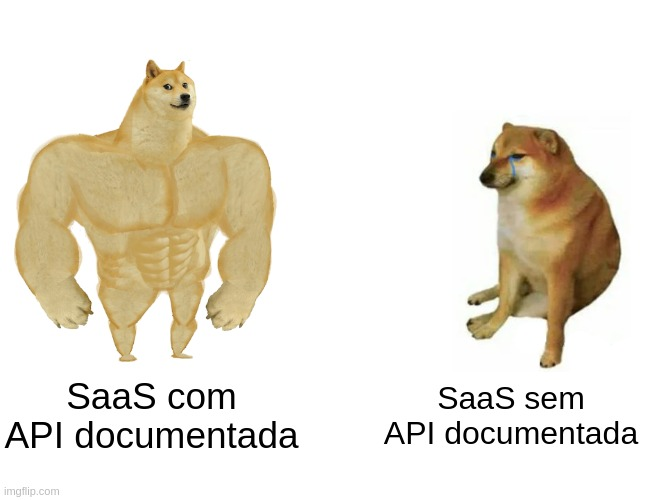
\includegraphics[width=0.5\textwidth]{assets/imagem-do-dia/saas-api-meme.jpeg}}

	\end{figure}
\end{frame}

\footlinecolor{}

\backmatter
\end{document}
